%!TEX root = ../dissertation.tex

\chapter{Results and Discussion}
\label{cha4:results}

This chapter presents the results obtained for various experiments, in which several aspects are put to test. First the three algorithms are tested under the simulator, for rotation estimation error with the saccades ranging between two different amplitudes, for variable pixel noise, for variable distance to the furthest point from the camera and for robust estimation. Afterwards, the algorithms and the \acrshort{imu} are tested on the real eye prototype, for rotation estimation error and robust estimation. After each experiment topic there is a small discussion on the results. In the end of the chapter, there are final remarks summarizing everything.

The coordinate system convention used throughout this chapter is the computer vision one mentioned in section \ref{cha2:represent}. 

\section{Simulator}
As in Figure \ref{cha1:sec1:fig:curr_eye_model}, the current eye prototype contains a baseline length of $53.7 \ mm$ on the torsional axis. To make the comparisons easier, this baseline was also used in the simulator.
\subsection{Rotation estimation error}
\label{reiovniorevn}
In Experiment 1, to simulate the saccade amplitudes, the variance used on the Gaussian distribution was $4 \degree$, which is realistic in relation to the human eye. In experiment 2, the variance was $15 \degree$, in order to understand how the estimation algorithm works in wider amplitude ranges.
\subsubsection{Simulation Parameters}
The following parameters were used to run the simulation. Zmax and Zmin refer to the range in which points are simulated explained on section \ref{rienreive}.
\begin{itemize}
	\item Maximum number of matches : $30$
	\item Maximum error: $0.05 \ m$
	\item False number of matches : $10 \%$ of maximum number of matches
	\item Good number of matches : $50 \%$ of the maximum number of matches
	\item Gaussian Noise $\sigma^2$ : $10 \ px$
	\item Number of saccades: $45$
	\item Zmin : $0.05 m$
	\item Zmax : $5 m$
\end{itemize}
The lines on the graphs below represent the best fitting of the points.
\subsubsection{Experiment 1 - Saccade amplitudes generated with $\sigma^2 = 4 \degree $}
Figures \ref{cha5:sec1:10anglex}, \ref{cha5:sec1:10angley} and \ref{cha5:sec1:10anglez}, show the error, computed according to \ref{firenr}, from the estimation of the rotation per saccade component along the horizontal, vertical and torsional axis, respectively. The saccades were generated randomly around a specific axis with a normal distribution with variance $\sigma^2 = 4 \degree$. Table \ref{cha5:sec1:10angleaxist}, shows the corresponding mean error in degrees per axis for each of the methods.\\

\begin{minipage}{0.5\textwidth}
	\centering
	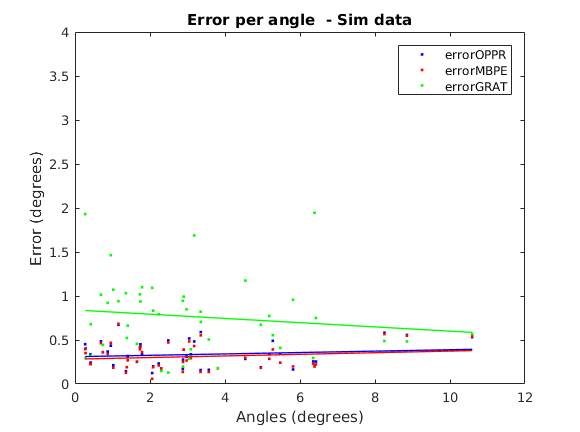
\includegraphics[width=\textwidth]{images/sim/10anglex.png}
	\captionof{figure}{Error as function of amplitude (in degrees) under simulation on the horizontal axis.}
	\label{cha5:sec1:10anglex}
\end{minipage}
\begin{minipage}{0.5\textwidth}
	\centering
	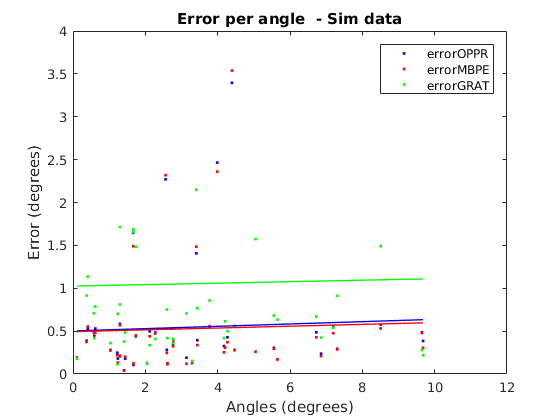
\includegraphics[width=\textwidth]{images/sim/10angley.png}
	\captionof{figure}{Error as function of amplitude (in degrees) under simulation on the vertical axis.}
	\label{cha5:sec1:10angley}
\end{minipage}
\begin{figure}[h]
	\centering
	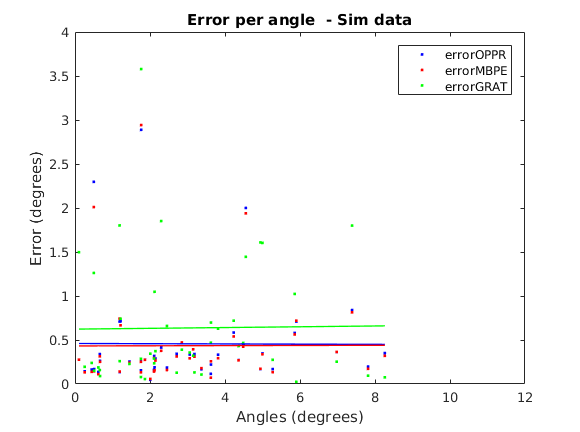
\includegraphics[width=0.5\textwidth]{images/sim/10anglez.png}
	\captionof{figure}{Error as function of amplitude (in degrees) under simulation on the torsional axis.}
	\label{cha5:sec1:10anglez}
\end{figure}
\begin{table}
	\centering
	\begin{tabular}{| l | l | l | l |}
		\hline
		Method & X Mean & Y Mean & Z Mean \\
		\hline
		OPPR &  0.33 \degree & 0.54 \degree & 0.46 \degree \\
		\hline
		MBPE &  0.31 \degree & 0.52 \degree & 0.44 \degree\\
		\hline
		GRAT &  0.77 \degree & 1.05 \degree & 0.64 \degree\\ 
		\hline
	\end{tabular}
	\captionof{table}{Mean error (in degrees) per method and per axis for saccade amplitudes with variance $\sigma^2 = 4 \degree $ under simulation.}
	\label{cha5:sec1:10angleaxist}
\end{table}		

Figure \ref{cha5:sec1:10angle} shows the error from the estimation of the rotation per saccade amplitudes randomly executed around all three axes, simultaneously. Table \ref{cha5:sec1:10anglet} shows the mean error and standard deviation for this experiment for each of the methods.\\

\begin{minipage}{0.5\textwidth}
	\centering
	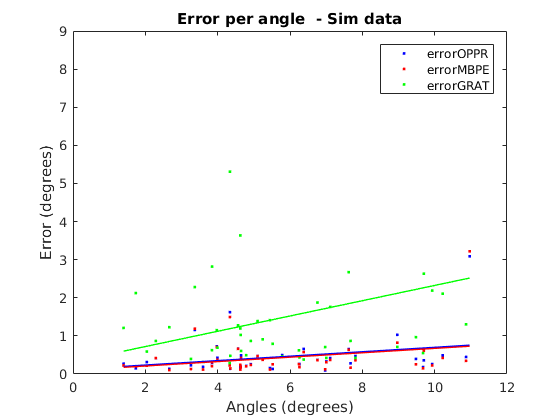
\includegraphics[width=\textwidth]{images/sim/10angle.png}
	\captionof{figure}{Error as function of amplitude (in degrees) under simulation for saccade amplitudes with variance $\sigma^2 = 4 \degree $}
	\label{cha5:sec1:10angle}
\end{minipage}
\begin{minipage}{0.5\textwidth}
	\centering
	\begin{tabular}{| l | l | l |}
			\hline
			Method & Mean & Standard Deviation \\
			\hline
			OPPR &  0.45 \degree & 0.49 \degree \\
			\hline
			MBPE &  0.42 \degree & 0.50 \degree \\
			\hline
			GRAT &  1.47 \degree & 1.76 \degree \\ 
			\hline
	\end{tabular}
	\captionof{table}{Mean error and standard deviation (in degrees) of the experiment on the left per each method tested for saccade amplitudes with variance $\sigma^2 = 4 \degree $ under simulation.}
	\label{cha5:sec1:10anglet}
\end{minipage}\\

Robust estimation was applied to filter out wrong matches, which amounted to $15.55 \%$ of them from the whole set of matches.

\subsubsection{Experiment 2 - Saccade amplitudes generated with $\sigma^2 = 15 \degree $}

Just like Experiment 1, Figure \ref{cha5:sec1:45angle} shows the error per  component axis in degrees for random saccades around all axes, simultaneously, generated by a normal distribution with variance $\sigma^2 = 15 \degree $. Table \ref{cha5:sec1:45anglet} presents the respective mean error and standard deviation. Robust estimation detected a $ 22.55 \%$ of bad matches.

\begin{minipage}{0.5\textwidth}
	\centering
	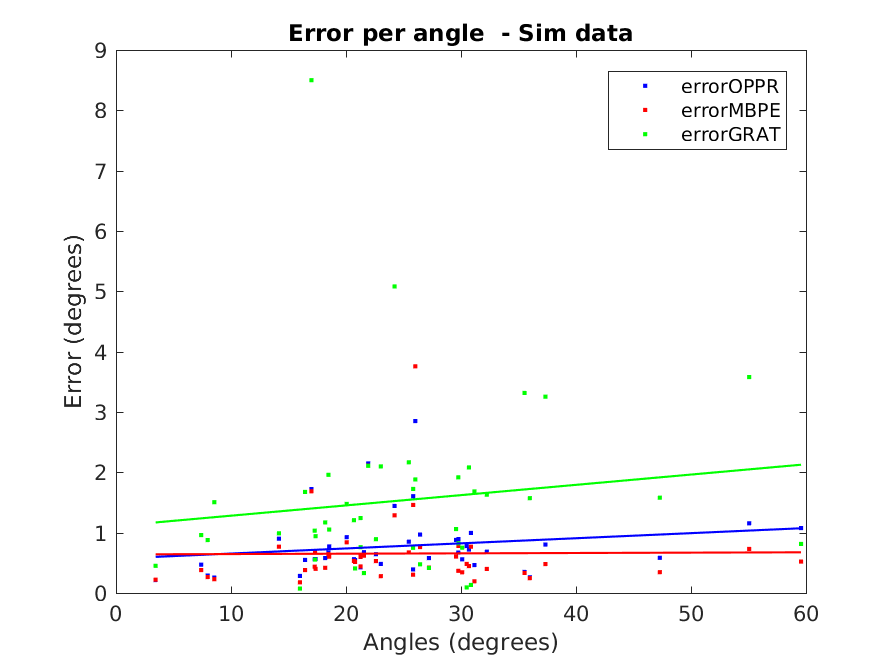
\includegraphics[width=\textwidth]{images/sim/45angle.png}
	\captionof{figure}{Error as function of amplitude (in degrees) under simulation for saccade amplitudes with variance $\sigma^2 = 15 \degree $}
	\label{cha5:sec1:45angle}
\end{minipage}
\begin{minipage}{0.5\textwidth}
	\centering
	\begin{tabular}{| l | l | l |}
		\hline
		Method & Mean & Standard Deviation \\
		\hline
		OPPR &  0.77 \degree & 0.49 \degree \\
		\hline
		MBPE &  0.65 \degree & 0.60 \degree \\
		\hline
		GRAT &  1.53 \degree & 1.43 \degree \\ 
		\hline
	\end{tabular}
	\captionof{table}{Mean error and standard deviation (in degrees) of the experiment on the left per each method tested for saccade amplitudes with variance $\sigma^2 = 15 \degree $ under simulation.}
	\label{cha5:sec1:45anglet}
\end{minipage}\\

\subsubsection{Overview}

Doing the saccades per isolated axis on Experiment 1, demonstrated that there is not a significant difference in the error around a specific coordinate by looking at Table \ref{cha5:sec1:10angleaxist}. Given that, the experiments can comfortably be executed with random saccades around all axis at the same time, which represents the real human eye more accurately.

Table \ref{cha5:sec1:10anglet} and Figure \ref{cha5:sec1:10angle} on Experiment 1, show that for angles under $ 12 \degree $ the mean error is under $0.5 \degree$ for the best two methods, \acrshort{oppr} and \acrshort{mbpe}, whereas for \acrshort{grat} the error is greater. \acrshort{mbpe} seems to be the best method in this case. The standard deviation is comparable to the mean for all the methods.

In Table \ref{cha5:sec1:45anglet} and Figure \ref{cha5:sec1:45angle} (Experiment 2), the conditions are all the same except for the amplitude range. Still \acrshort{mbpe} and \acrshort{oppr} continue to be superior to \acrshort{grat}, this time having \acrshort{oppr} become worse as the saccade amplitude increases. This may be due to the fact that for a bigger saccade, the associated translation creates a larger contribution that is not compensated when using \acrshort{oppr}. Overall, the error increases as the saccade amplitude increases proportionally for all methods.

There might be several reasons as to why \acrshort{grat} performs worse than the other algorithms. Because the baseline length is small, the skew translation matrix, that generates the essential matrix together with the rotation, expressed in \ref{sec2:eq:fundm3}, will have values very close to zero, that during intermediate calculus in the minimization can reduce the accuracy of the estimation. Other reason could be that, because the depth, $\lambda$, is not being estimated, in contrast to \acrshort{mbpe} (see \ref{fiorenfe}), the leeway to estimate the rotation is reduced, ending up with a poorer guess.
 

\subsection{Variable noise}
To test how measurement noise affects the algorithms, all the same parameters as the previous section were kept and the amplitude of the saccades was set to a variance of $4 \degree$ again, while the added noise varies from $0$ to $100 \ px$. 
\subsubsection{Simulation Parameters}
\begin{itemize}
	\item Maximum number of matches : $30$
	\item Maximum error: $0.05 \ m$
	\item Good number of matches : $50 \%$ of the maximum number of matches
	\item False number of matches : $10 \%$ of maximum number of matches
	\item Noise $\sigma^2$ : $0-100 \ px$ incrementing $10 \ px$ per iteration
	\item Number of saccades: $45$
	\item Zmin : $0.05 m$
	\item Zmáx : $5 m$
	\item Saccade amplitude $\sigma^2 : 4 \degree $
\end{itemize}
Figure \ref{cha5:sec1:noise} shows how the mean error increases with the amount of pixel noise. It can be seen that \acrshort{grat} is more sensitive to measurement noise than the two methods.
\begin{figure}[ht]
	\centering
	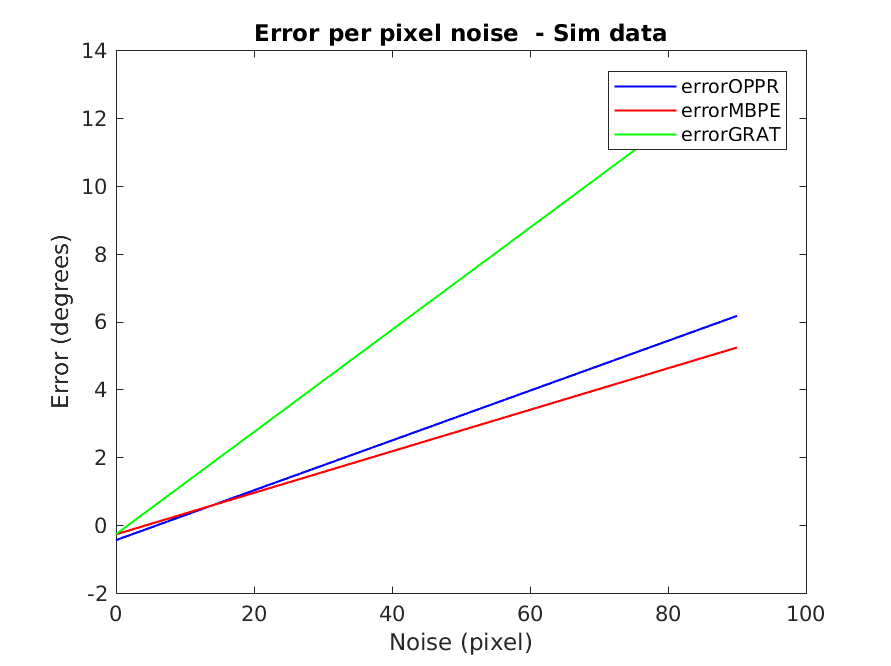
\includegraphics[width=0.5\textwidth]{images/sim/noise.png}
	\captionof{figure}{Error (in degrees) as function of the amount of noise in the simulated image (in pixels).}
	\label{cha5:sec1:noise}
\end{figure}

\subsection{Variable distance}
To see how the distance from the furthest object to the camera influences with the estimation, a simulation with the following parameters was run, with a varying distance from $5 \ cm$ to $10 \ m$.
\subsubsection{Simulation Parameters}
\begin{itemize}
	\item Maximum number of matches : $30$
	\item Maximum error: $0.05 \ m$
	\item Good number of matches : $50 \%$ of the maximum number of matches
	\item False number of matches : $10 \%$ of maximum number of matches
	\item Noise $\sigma^2$ : $10 \ px$ incrementing $10 \ px$ per iteration
	\item Number of saccades: $45$
	\item Z : $0.05 m$ to $10 \ m$ incrementing $1 \ m$ per iteration.
	\item Saccade amplitude $\sigma^2 : 4 \degree $
\end{itemize}
The further away the points are, the more approximate to a pure rotation the movement becomes as explained in section \ref{fipewnf}.
Figure \ref{cha5:sec1:depthh} exhibits the error in degrees according to the the distance to the furthest points from the camera. \acrshort{oppr} and \acrshort{mbpe}, improve with distance, probably due to rejecting image sections, which will be studied in more detail on next section. \acrshort{grat} makes use of translation to get a good estimation, so it doesn't really gain anything from distance, except for a better initialization given by \acrshort{oppr}.
\begin{figure}[ht]
	\centering
	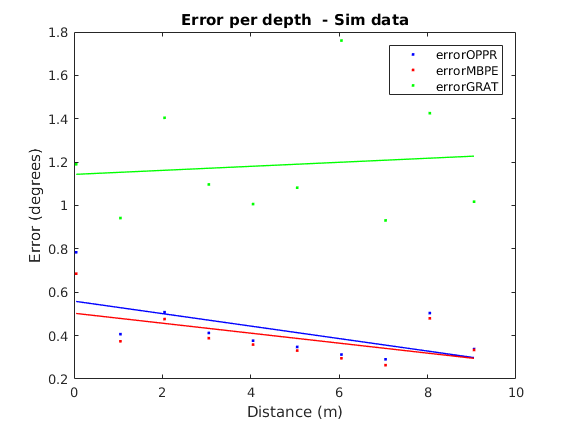
\includegraphics[width=0.5\textwidth]{images/sim/depthh.png}
	\captionof{figure}{Error (in degrees) as function of distance to the camera in the simulated scene in meters.}
	\label{cha5:sec1:depthh}
\end{figure}	

\subsection{Effect of rejecting image sections}

To understand how by doing robust estimation with \acrshort{oppr}, the rejection of image sections is affecting the estimation of the orientation, a simulation was run with the following parameters.

\subsubsection{Simulation Parameters}
\begin{itemize}
	\item Maximum number of matches : $30$
	\item Maximum error: $0.05 \ m$
	\item Good number of matches : $50 \%$ of the maximum number of matches
	\item False number of matches : $0 \%$ of maximum number of matches
	\item Noise $\sigma^2$ : $0 px$
	\item Number of saccades: $45$
	\item Zmin : $0.05 m$
	\item Zmáx : $5 m$
	\item Saccade amplitude $\sigma^2 : 15 \degree $
\end{itemize}

By having no noise or false matches to eliminate, the effect of rejecting image section is easier to study, under simulation. The variance for saccade amplitude generation is now $\sigma^2 = 15 \degree $ to emphasize the effect, as bigger translations are executed.

\subsubsection{Experiment 1 - Without robust estimation}
Figure \ref{cha5:sec1:withoutr} and Table \ref{cha5:sec1:withoutrt} correspond to running the algorithms without robust estimation.\\

\begin{minipage}{0.5\textwidth}
	\centering
	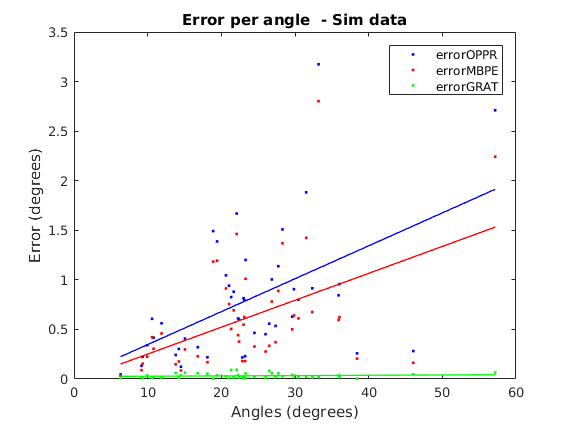
\includegraphics[width=\textwidth]{images/sim/withoutransac.png}
	\captionof{figure}{Error per saccade amplitude (in degrees) under the simulation \textbf{without} robust estimation.}
	\label{cha5:sec1:withoutr}
\end{minipage}
\begin{minipage}{0.5\textwidth}
\begin{tabular}{| l | l | l |}
	\hline
	Method & Mean & Standard Deviation \\
	\hline
	OPPR &  0.79 \degree & 0.63 \degree \\
	\hline
	MBPE &  0.61 \degree & 0.56 \degree \\
	\hline
	GRAT &  0.03 \degree & 0.02 \degree \\ 
	\hline
\end{tabular}
\captionof{table}{Mean error and standard deviation (in degrees) of the experiment on the left per each method tested \textbf{without} robust estimation.}
\label{cha5:sec1:withoutrt}
\end{minipage}\\

\subsubsection{Experiment 2 - With robust estimation}
Figure \ref{cha5:sec1:withr} and Table \ref{cha5:sec1:withrt} were ran with robust estimation.\\
\begin{minipage}{0.5\textwidth}
	\centering
	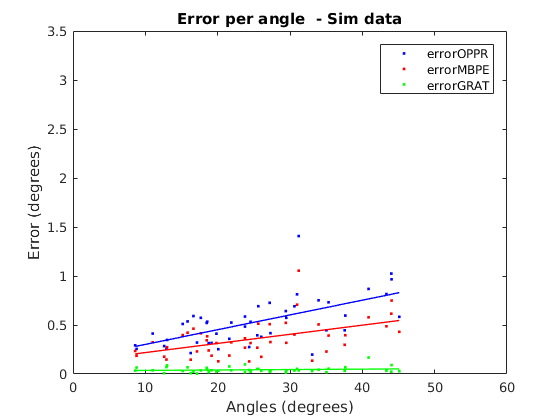
\includegraphics[width=\textwidth]{images/sim/withransac.png}
	\captionof{figure}{Error per saccade amplitude (in degrees) under the simulation \textbf{with} robust estimation.}
	\label{cha5:sec1:withr}
\end{minipage}
\begin{minipage}{0.5\textwidth}
\begin{tabular}{| l | l | l |}
	\hline
	Method & Mean & Standard Deviation \\
	\hline
	OPPR &  0.53 \degree & 0.24 \degree \\
	\hline
	MBPE &  0.36 \degree & 0.18 \degree \\
	\hline
	GRAT &  0.04 \degree & 0.03 \degree \\ 
	\hline
\end{tabular}
\captionof{table}{Mean error and standard deviation (in degrees) of the experiment on the left per each method tested \textbf{with} robust estimation.}
\label{cha5:sec1:withrt}
\end{minipage}\\

\subsubsection{Overview}

As it was mentioned on section \ref{fipewnf}, doing \acrshort{ransac}+\acrshort{oppr} for robust estimation, yields point matches that are more approximate to a pure rotation.

When looking at the results from Experiment 1 and 2, it's possible to see that it has slightly improved by using robust estimation for the methods \acrshort{oppr} and \acrshort{mbpe}. For the former, this was very expected, as it is most accurate when dealing with pure rotations, as for \acrshort{mbpe} by taking \acrshort{oppr} as an initialization parameter, it is normal to also have its results improved. \acrshort{grat} has a really small error now compared to the results in Figure \ref{cha5:sec1:45angle}, which probably indicates that it is extremely sensitive to Gaussian noise in the images, that is not present here. This in fact makes sense, as this algorithm uses pixel coordinates directly to estimate the rotation.

\section{Real System}
\subsection{Data collection}
To test the algorithms under the real system, 10 images of a scenery, with the setup mentioned on \ref{cha4:sec3:eyescheme}, were took with and without a chessboard at the same time as the \acrshort{imu} collected the current orientation of the eye prototype, for each experiment. Joining the images/orientations with each other made up to 45 different saccades. 
\subsection{Rotation estimation error}
\label{fefwefesxs}
The algorithms were then run with the following parameters.
\subsubsection{System Parameters}
\begin{itemize}
	\item Maximum number of matches : $30$
	\item Maximum error: $0.05 \ m$
	\item Good number of matches : $50 \%$ of the maximum number of matches
	\item Zmin : $0.05 m$
	\item Zmáx : $5 m$
	\item Saccade amplitude : random
\end{itemize}

The lines on the graphs below represent the best fitting of the points.
\subsubsection{Experiment 1}
In experiment 1, all the 45 rotations obtained from the ground truth were valid to be analyzed.\\
Figure \ref{cha5:sec1:r1angle} presents the error per saccade amplitude on the real system in degrees for the camera, and Figure \ref{cha5:sec1:r1angleimu} shows the same for the \acrshort{imu}. Table \ref{cha5:sec1:r1anglet} displays the corresponding mean error and standard deviation for each method and for the \acrshort{imu}.

Robust estimation applied to the images detected $ 94.96 \%$ of wrongly paired matches. \\

\begin{minipage}{0.5\textwidth}
\centering
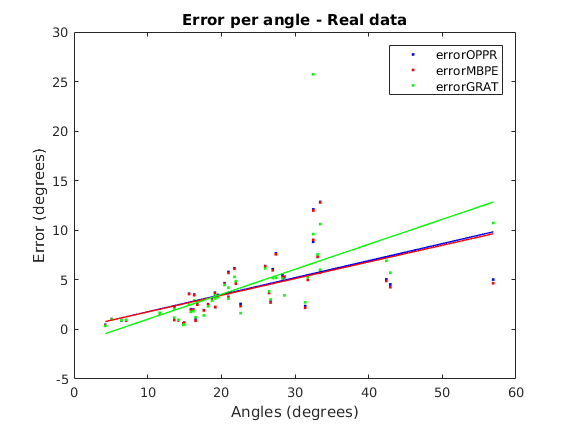
\includegraphics[width=\textwidth]{images/sim/r1angle.png}
\captionof{figure}{Error per saccade amplitude (in degrees) under the real system for the camera estimation.}
\label{cha5:sec1:r1angle}
\end{minipage}
\begin{minipage}{0.5\textwidth}
\centering
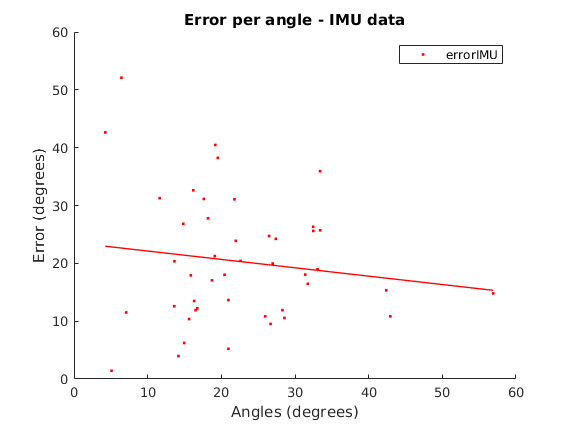
\includegraphics[width=\textwidth]{images/sim/r1angleimu.png}
\captionof{figure}{Error per saccade amplitude (in degrees) under the real system for the \acrshort{imu} estimation.}
\label{cha5:sec1:r1angleimu}
\end{minipage}\\

\begin{table}[ht]
	\centering
\begin{tabular}{| l | l | l |}
	\hline
	Method & Mean & Standard Deviation \\
	\hline
	OPPR &  3.90 \degree & 2.75 \degree \\
	\hline
	MBPE &  3.83 \degree & 2.75 \degree \\
	\hline
	GRAT &  4.13 \degree & 4.09 \degree \\ 
	\hline
	IMU &  20.34 \degree & 10.85 \degree \\ 
	\hline
	IMU without the vertical axis &  11.79 \degree & 3.57 \degree \\ 
	\hline
\end{tabular}
\captionof{table}{Mean error and standard deviation (in degrees) of the experiment on Figure \ref{cha5:sec1:r1angle} and \ref{cha5:sec1:r1angleimu} per each method tested.}
\label{cha5:sec1:r1anglet}
\end{table}

\begin{figure}[ht]
	\centering
	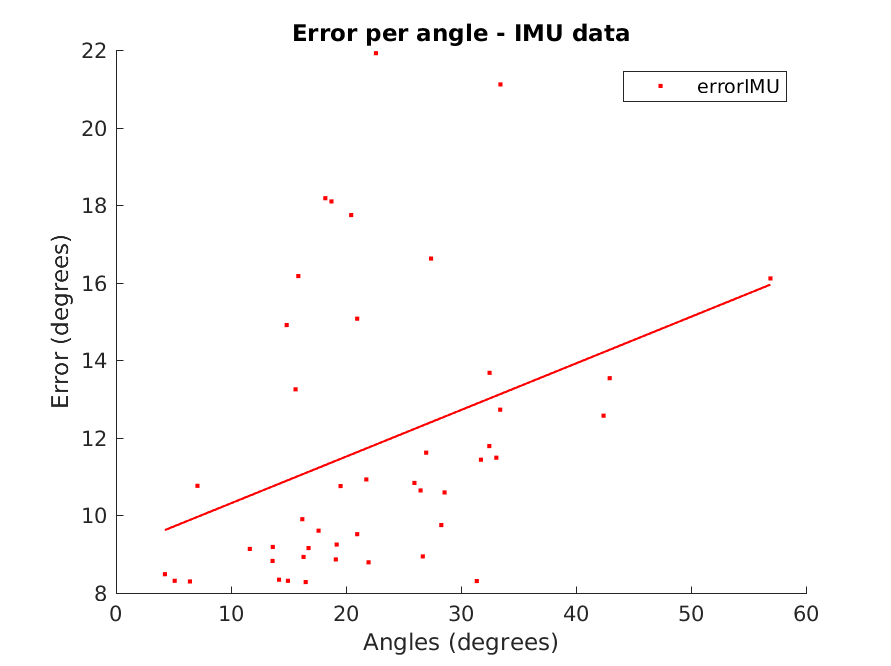
\includegraphics[width=0.5\textwidth]{images/sim/imuerrorissue.png}
	\captionof{figure}{The same experiment as \ref{cha5:sec1:r1angleimu} but only visualizing the error on the horizontal and torsional axis per saccade amplitude (in degrees).}
	\label{cha5:sec1:imuerrorissue}
\end{figure}


\subsubsection{Experiment 2}
In experiment 2, 13 of the saccades were invalid, thus only 32 are  assessed. Figure \ref{cha5:sec1:r2angle} and \ref{cha5:sec1:r2angleimu} exhibit the error per saccade amplitude in degrees for the camera estimation and for the \acrshort{imu} estimation, respectively. Table \ref{cha5:sec1:r2anglet} shows the corresponding mean error and standard deviation for each method and the \acrshort{imu}.

Robust estimation detected a $ 93.68 \%$ of bad matches.

\begin{minipage}{0.5\textwidth}
	\centering
	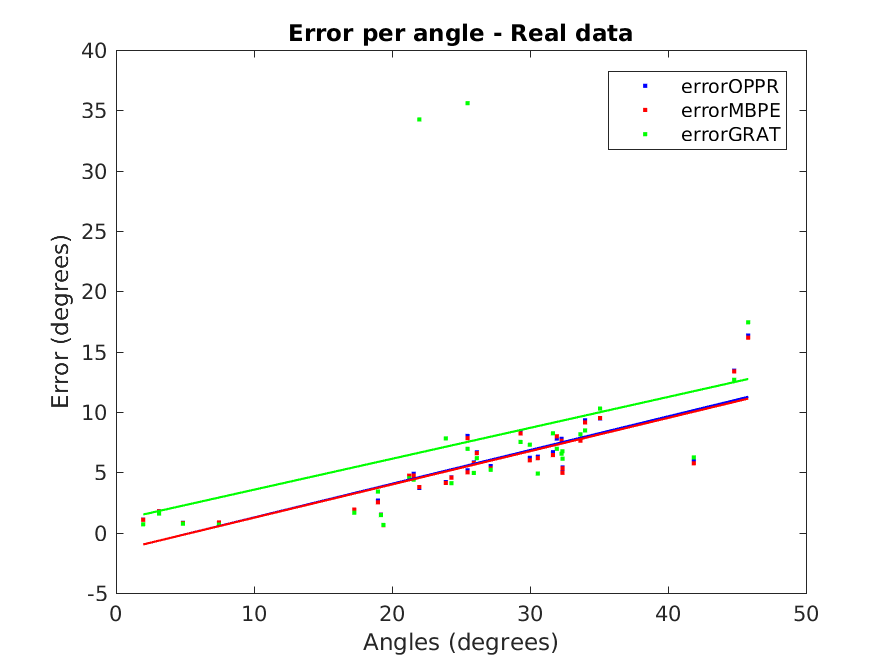
\includegraphics[width=\textwidth]{images/sim/r2angle.png}
	\captionof{figure}{Error per saccade amplitude (in degrees) under simulation for the camera estimation.}
	\label{cha5:sec1:r2angle}
\end{minipage}
\begin{minipage}{0.5\textwidth}
	\centering
	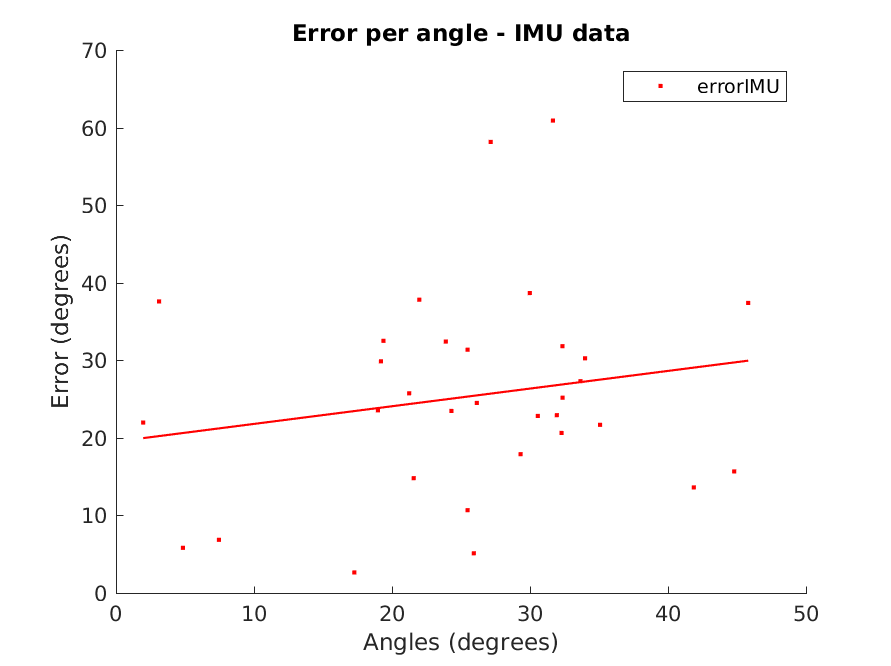
\includegraphics[width=\textwidth]{images/sim/r2angleimu.png}
	\captionof{figure}{Error per saccade amplitude (in degrees) under simulation for the \acrshort{imu} estimation.}
	\label{cha5:sec1:r2angleimu}
\end{minipage}\\

\begin{table}
	\centering
	\begin{tabular}{| l | l | l |}
		\hline
		Method & Mean & Standard Deviation \\
		\hline
		OPPR &  5.63 \degree & 3.43 \degree \\
		\hline
		MBPE &  5.55 \degree & 3.40 \degree \\
		\hline
		GRAT &  7.57 \degree & 7.79 \degree \\ 
		\hline
		IMU &  25.36 \degree & 13.13 \degree \\ 
		\hline
	\end{tabular}
	\captionof{table}{Mean error and standard deviation (in degrees) of the experiment on Figure \ref{cha5:sec1:r2angle} and \ref{cha5:sec1:r2angleimu} per each method tested}
	\label{cha5:sec1:r2anglet}
\end{table}

\subsubsection{Overview}

Both Experiments 1 and 2 were the same but with two different sets of images, in order to validate the results.

Similarly to the simulation results in section \ref{reiovniorevn}, as seen on Figures \ref{cha5:sec1:r1angle} and \ref{cha5:sec1:r2angle}, \acrshort{oppr} and \acrshort{mbpe} keep being better than \acrshort{grat}.

When comparing the camera estimation algorithms, in Experiment 1, the best mean error for the camera is $3.83 \degree $, from \acrshort{mbpe} with a standard deviation of $2.75 \degree$. This error is probably due to noise in the image or even false matches that were not filtered out in the robust estimation. As it is real data, there is always noise associated and imposing stricter parameters for the quantity of good matches or maximum error for \acrshort{ransac} (see section \ref{rnfireonce}) will eventually not yield enough point matches to work with.

Experiment 1's estimation errors are smaller than Experiment 2, that is because the points in 1 are more concentrated around smaller angles where the error is less.

The \acrshort{imu} estimation results, shown on Figures \ref{cha5:sec1:r1angleimu} and \ref{cha5:sec1:r2angleimu} and on the respective Tables, manifest a huge error in relation to the camera. Besides that, this error doesn't seem to have a pattern like the camera's, where the error increases with the saccade amplitude. This outcome may be caused by unstable measurements during the experiment, as the \acrshort{imu} needs to stabilize its position for some time until it gives a correct orientation. It could also be justified by the drift specially when associated to rotations around the vertical axis (as it cannot use the force of gravity for the measurements). This last motivation can be backed up by Figure \ref{cha5:sec1:imuerrorissue}, that shows the same as Figure \ref{cha5:sec1:r1angleimu} without the rotation estimation around the vertical axis, presenting half the error as previously and an increasing pattern.


\subsection{Effect of robust estimation}

Figure \ref{cha5:sec1:r1angleransac} and Table \ref{cha5:sec1:r1angleransact} show the same Experiment 1 described in section \ref{fefwefesxs}, but without applying robust estimation. The mean error went up a lot compared to the same Experiment using \acrshort{ransac}, most probably due to false matches.\\

\begin{minipage}{0.5\textwidth}
	\centering
	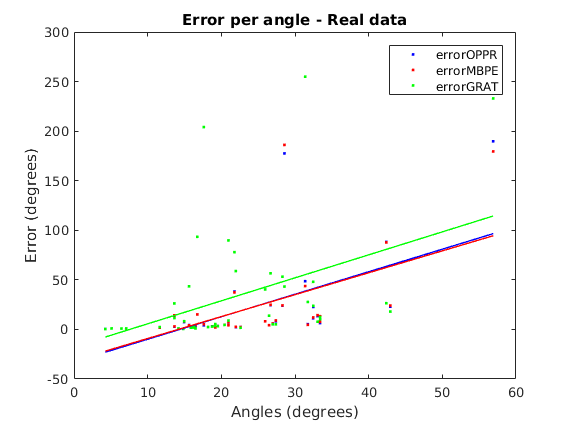
\includegraphics[width=\textwidth]{images/sim/r1angleransac.png}
	\captionof{figure}{Error per saccade amplitude (in degrees) under the real system without robust estimation.}
	\label{cha5:sec1:r1angleransac}
\end{minipage}
\begin{minipage}{0.5\textwidth}
	\centering
	\begin{tabular}{| l | l | l |}
		\hline
		Method & Mean & Standard Deviation \\
		\hline
		OPPR &  18.07 \degree & 38.47 \degree \\
		\hline
		MBPE &  18.09 \degree & 38.17 \degree \\
		\hline
		GRAT &  34.24 \degree & 57.54 \degree \\ 
		\hline
	\end{tabular}
	\captionof{figure}{Error per saccade amplitude (in degrees) under the real system without robust estimation.}
	\label{cha5:sec1:r1angleransact}
\end{minipage}\\

\subsection{Computational time}

When using the created C++ library (see section \ref{diwefneoinfof}), the computational times seen on Table \ref{cha5:sec1:speed} were obtained for each of the processes that have to be executed to estimate the eye prototype's orientation and for the \acrshort{imu} estimation.

\begin{table}[ht]
	\centering
	\begin{tabular}{| l | l | l |}
		\hline
		Process & Time \\
		\hline
		Image Capture & $120 \ ms$  \\
		\hline
		Undistort + Find Keypoints &   $421 \ ms$ \\
		\hline
		Find Matches & $16 \ ms$ \\ 
		\hline
		Robust Estimation & $10 \ ms$ \\ 
		\hline
		OPPR & $13\mathrm{e}{-2} \ ms$ \\ 
		\hline
		MBPE & $212 \ ms$ \\ 
		\hline
		GRAT & $51 \ ms$ \\ 
		\hline
		IMU Estimation &  $40\mathrm{e}{-4} \ ms$ \\ 
		\hline
	\end{tabular}
	\captionof{table}{Computational time for each of the necessary processes to estimate the orientation of the eye prototype in C++.}
	\label{cha5:sec1:speed}
\end{table}

Obviously, the \acrshort{imu} takes much less time estimating the orientation than the camera. For the quickest algorithm, \acrshort{oppr}, the total amount of time taken is $567 \ ms$. 

\subsection{Final Remarks}

\begin{itemize}
	\item \acrshort{oppr} is the fastest and the most light-weight of the camera estimation methods. Because it ignores the translation associated to the eye prototype rotations, it performs better when the movement is closer to pure rotations. If the scenery is very far way, the algorithm improves. Using \acrshort{ransac}+\acrshort{oppr} to filter out point matches also refines the estimation.
	
	\item \acrshort{mbpe} seemed to be the best camera algorithm out of all the Experiments. However, because it has to estimate both the three Euler angles and depth, $\lambda$, for each point match, a total of ($2+n$) parameters, it is the one that takes the longest. It improves when \acrshort{oppr} improves, as it highly depends on the initialization.
	
	\item \acrshort{grat} did the worst in the Experiments and proved to be very sensitive to pixel noise in the image. It does better when associated to bigger saccade amplitudes, as they have more translation associated. It has a big downside, which is not working for pure rotations, as mentioned on section \ref{fjeopfe}.
	
	\item \acrshort{imu} estimation is the fastest method but the error is much higher than in the camera algorithms, most probably due to rotation around the vertical axis.	
	
\end{itemize}

Having said that, the most accurate method is \acrshort{mbpe}. 

















